\section{Introduction}
\label{sec:introduction}

Let $G_1=(V,E_1)$ and $G_2=(V,E_2)$ be planar graphs.  A
\emph{simultaneous embedding with fixed edges} (\SEFE) is a pair of planar
drawings that represent every vertex by the same point and every edge of
$H=(V,E_1\cap E_2)$ by the same curve.  Edges belonging exclusively to
different input graphs may cross.  The distinction from drawing the union
$G_1\cup G_2$ planarly is essential: the union need not be planar.

For three or more input graphs the problem is
NP-complete~\cite{gjpss06}.  For two input graphs its complexity has
remained open; it is stated as an open problem in recent
work~\cite{fpr,isaac,ramsey}.  The general decision problem has resisted the
usual planarity-decomposition techniques.  The connected-common-graph case
was first solved in polynomial time by Fulek and T\'oth~\cite{atomic}, and
in quadratic time by Synchronized Planarity~\cite[Theorem~16]{bfr}, but
disconnected common graphs carry information not determined by local
rotations.  Even when the two
colours agree on the rotation of every common edge, a component of $H$ may
occupy different faces of another common component.  These relative
positions interact at common cutvertices and at separation pairs of the
input graphs~\cite{brdisconnect,bkr}.

\begin{theorem}\label{thm:main}
There is a deterministic polynomial-time algorithm which, given two planar
graphs $G_1,G_2$ on the same vertex set, decides whether they admit a
simultaneous embedding with fixed edges.  On a positive instance it
constructs compatible combinatorial embeddings, including the relative
positions of all connected components of their common graph.  No
connectivity, degree, or block restriction is imposed on the common graph.
\end{theorem}

The proof is constructive.  With
\[
 N=|V|+|E_1|+|E_2|,
\]
a deliberately generous bound for the algorithm presented here is
$O((N+1)^{60})$.  We make no attempt to optimize this exponent.

\paragraph{Face compatibility.}
The first step separates the choice of block embeddings from their
assembly.  Suppose an oriented planar embedding has already been selected
for every biconnected block of each input graph.  Compatible orders of the
common darts at a vertex are necessary, but not by themselves sufficient.
For each common block $K$ and each component $Z$ of
$(G_1\cup G_2)-V(K)$, all of $Z$ must occupy one face of $K$.  That face
must be incident with every attachment of $Z$ and must agree with the
positions of the pieces of $Z$ already prescribed within the colour
blocks containing $K$.

We prove that these requirements are also sufficient
(Theorem~\ref{rep:thm:repair}).  The local repair is described by a tree
whose nodes represent common blocks and the regions between them.  Its
contour constructs compatible orders without changing any prescribed
colour-block embedding.  The theorem applies to disconnected $H$, to
isolated common vertices, and to arbitrarily many common blocks meeting
at a cutvertex.

\paragraph{Face sectors rather than individual side bits.}
The second step is to choose the colour-block embeddings subject to the
face requirements.  After the separation-pair preprocessing of
Bl\"asius--Karrer--Rutter~\cite[Lemmas~2--4 and Theorem~2]{bkr}, every
P-node of a common block has a known cyclic order up to reversal
(Section~\ref{gen:porders} treats a real common pole edge); see also
Fink--Pfretzschner--Rutter~\cite[Lemma~4(c)]{fpr}.  A binary order choice,
however, does not remove the many possible faces between the expansions
of a P-node.

Let a common P-node have poles $p,q$ and reference directions
$e_0,\ldots,e_{k-1}$.  Its faces incident with both poles correspond to
the $k$ sectors between successive directions.  We retain a sector as one
variable with $k$ possible values instead of asking separately on which
side of several common cycles a component lies.  This is essential:
orientations of several triples at one freely permutable P-node need not
form an affine Boolean relation.

The crucial structural distinction is determined by the attachment set
$A_K(Z)=N_{G_1\cup G_2}(Z)\cap V(K)$.
\begin{itemize}[leftmargin=1.4em]
\item If $A_K(Z)=\{p,q\}$ for the poles of a common P-node, we keep the
      \emph{entire face name} of $Z$, and compare it directly with the face
      names of the relevant colour lobes.
\item Otherwise a new vertex adjacent to all of $A_K(Z)$ witnesses an
      eligible face of $K$.  We compare that face with the faces of the
      colour lobes using a fixed cycle basis of $K$.
\end{itemize}
\begin{figure}[t]
\centering
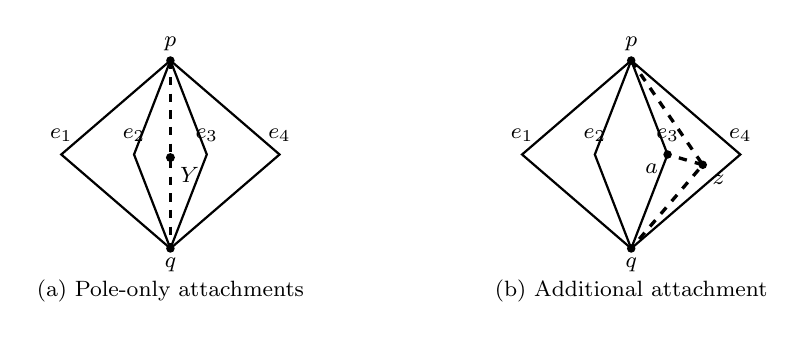
\begin{tikzpicture}[scale=.77, every node/.style={font=\footnotesize}]
  \begin{scope}[xshift=-3.8cm]
    \coordinate (p) at (0,1.55); \coordinate (q) at (0,-1.55);
    \foreach \x/\lab in {-1.8/1,-.6/2,.6/3,1.8/4} {
      \draw[thick] (p) -- (\x,0) -- (q);
      \node[above=1pt] at (\x,0) {$e_{\lab}$};
    }
    \fill (p) circle(2pt) node[above] {$p$};
    \fill (q) circle(2pt) node[below] {$q$};
    \coordinate (y) at (0,-.05);
    \draw[very thick, dashed] (p) -- (y) -- (q);
    \fill (y) circle(2.1pt) node[below right] {$Y$};
    \node at (0,-2.25) {(a) Pole-only attachments};
  \end{scope}
  \begin{scope}[xshift=3.8cm]
    \coordinate (p) at (0,1.55); \coordinate (q) at (0,-1.55);
    \foreach \x/\lab in {-1.8/1,-.6/2,.6/3,1.8/4} {
      \draw[thick] (p) -- (\x,0) -- (q);
      \node[above=1pt] at (\x,0) {$e_{\lab}$};
    }
    \coordinate (z) at (1.18,-.17);
    \draw[very thick, dashed] (p) -- (z) -- (q);
    \draw[very thick, dashed] (z) -- (.6,0);
    \fill (.6,0) circle(2pt) node[below left] {$a$};
    \fill (z) circle(2pt) node[below right] {$z$};
    \fill (p) circle(2pt) node[above] {$p$};
    \fill (q) circle(2pt) node[below] {$q$};
    \node at (0,-2.25) {(b) Additional attachment};
  \end{scope}
\end{tikzpicture}
\caption{Schematic face choices around a common P-node.  A component
attached only at $p,q$ may use any sector.  With an additional
attachment in the expansion $e_3$, its face must border that expansion.
Dashed edges denote private or auxiliary attachments; the drawing
shows one permissible placement in each case.}
\label{fig:sector-dichotomy}
\end{figure}

The only potentially nonaffine side observation in the second case comes
from an entire colour lobe attached at a common P-pair.  Since $Z$ has an
additional attachment, at most two sectors can contain it.  On this
restricted domain every side observation is a Boolean affine function.
Importantly, this restriction is applied \emph{in addition to}, not in
place of, the original face comparisons.

\paragraph{An exact constraint language.}
The resulting problem is a restricted extension of the Synchronized
Planarity problem of Bl\"asius--Fink--Rutter~\cite{bfr}.  A marked
P-vertex has one reference order of its marked darts, up to reversal, and
an unmarked dart may be assigned to a named sector.  Finite-domain
variables are related only by unary restrictions and partial bijections;
designated Boolean variables may also satisfy affine equations over
$\Ftwo$.  This language is tractable because a connected component of
partial-bijection constraints has at most two assignments as soon as it
contains a Boolean variable.  The residual Boolean system is solved by
Gaussian elimination.

The graph-theoretic work is to show that the ordinary Synchronized
Planarity reduction operations preserve these extra observations, in
\emph{both} witness directions.  We do this for encapsulation, joining,
propagation, the reordering of parallel expansions, self-pipes, and the
pipe-free terminal instance.  Two recurring tools are the injective
transport of a corner of a marked embedding subtree to a frontier sector
and the preservation of complete sector categories when whole expansion
intervals are reordered.  The case of two marked darts requires an
independent frame bit, even though their cyclic order is vacuous.

The three principal results are an assembly theorem
(Theorem~\ref{rep:thm:repair}), an exact compilation
(Theorem~\ref{gen:compilation}), and a solver for the complete-sector
constraint language (Theorem~\ref{cse:main}).  Their composition proves
Theorem~\ref{thm:main}.

\paragraph{Related work and scope.}
The preprocessing and the role of relative positions in disconnected
common graphs originate in~\cite{brdisconnect,bkr}.  Synchronized
Planarity gives a polynomial-time framework for several constrained
embedding problems~\cite{bfr}.  General Simultaneous PQ-Ordering is not
used as an algorithmic oracle: only its restricted variants are known to
be efficiently solvable~\cite{pqordering}.  Nor do we invoke Schaefer's
conjectured strong Hanani--Tutte theorem for
\SEFE{}~\cite[Conjecture~6.20]{schaefer}.  That conjecture is false:
Gutwenger, Mutzel and Schaefer~\cite{gms2014} turned the clustered-planarity
counterexamples of Fulek, Kyn\v{c}l, Malinovi\'c and P\'alv\"olgyi into
counterexamples to it (see~\cite[p.~6]{fkmp2015}
and~\cite[p.~137]{fps2017}).  The closest precedent for our engine is
Pfretzschner's extension of Synchronized Planarity by equations between
triple orientations, which solves \SEFE{} when both input graphs are
biconnected and have maximum degree four~\cite[Chapter~8]{pfretzschner};
the present language instead retains complete sector categories.
Carmesin and Turner~\cite{temporal} give a polynomial-time algorithm for
2-connected temporal sequences, and state that their framework also
resolves a rooted-tree variant of \SEFE{}.
A cycle-based repair construction for cactus
common graphs was developed in the preliminary manuscript~\cite{cactus};
we treat the results needed here directly, rather than importing that
manuscript as a theorem.

\paragraph{Organization.}
Section~\ref{sec:normalization} fixes conventions and proves the
normalization steps used subsequently.
Section~\ref{rep:section} proves the face-list assembly criterion.
Section~\ref{gen:section} constructs the constraint instance from an
arbitrary normalized SEFE instance.
Section~\ref{cse:section} gives the complete-sector solver, including the
inverse transformations.
Section~\ref{sec:composition} finishes the algorithm and its size bound.
Counterexamples to tempting weaker conditions and the finite checks are
separated into Appendix~\ref{sec:verification}.
